\section{Partial-fill Phase Analysis}


During the August to October 2019, the PPO is added into the LAB when the water level at 5100 mm (in PSUP coordinate). This is for the SNO+ partial-fill phase.


\subsection{Sky-shine Classifier}



A ``sky shine'' (SkyShine) classifier was developed by the collaboration to discriminate 


The SkyShine classifier aims to discriminate "sky shine" events from other backgrounds by looking at the ratio of hit counts in a middle z range and a low z range. It can also look at neck and high-z OWL PMT hits. The classifier's behavior for partial fill is studied using simulation.

\cite{skyshine}


\begin{figure}[!htb]
	\centering
	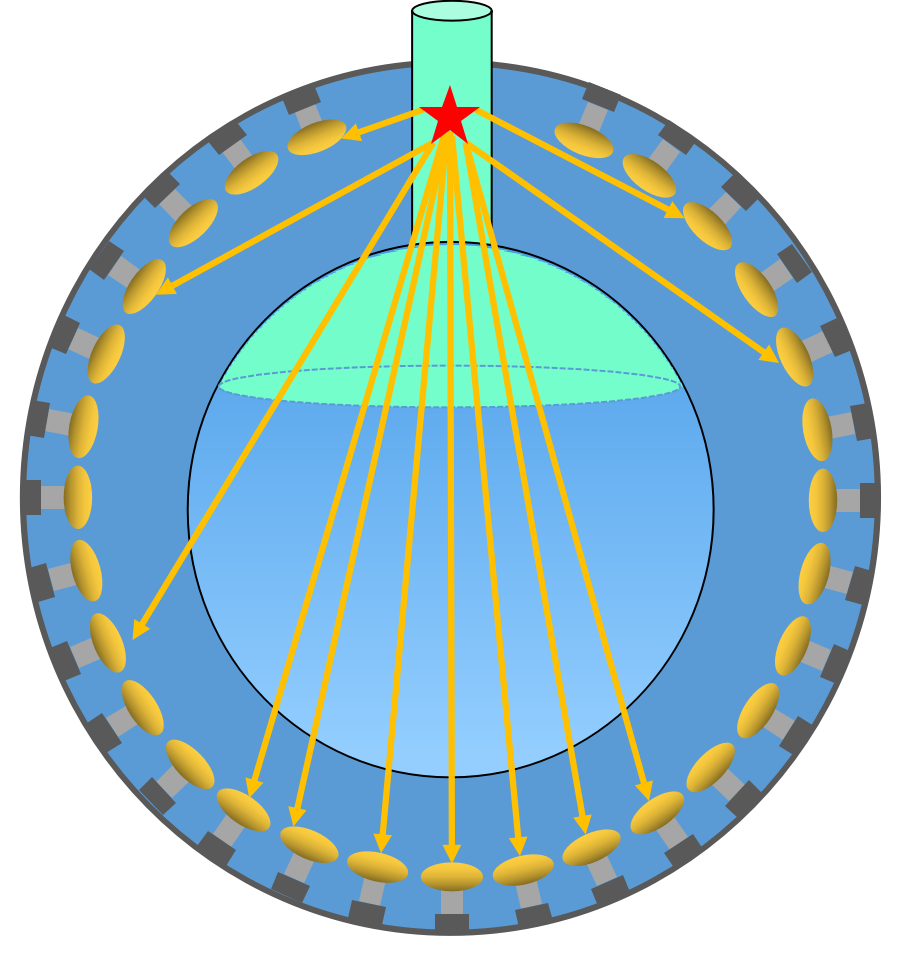
\includegraphics[width=6cm]{skyShine.png}
\caption{ An illustration for skyShine classifier, modified from \cite{skyshine}.}
	\label{drivecor}
\end{figure}



\subsection{Bi-Po Analysis}


\begin{tikzpicture}[node distance=2cm]
%%% settings
\tikzstyle{startstop} = [rectangle, rounded corners, minimum width=3cm, minimum height=1cm,text centered, draw=black, fill=red!30]
\tikzstyle{io} = [trapezium, trapezium left angle=70, trapezium right angle=110, minimum width=3cm, minimum height=1cm, text centered, draw=black, fill=blue!30]
\tikzstyle{process} = [rectangle, minimum width=3cm, minimum height=1cm, text centered, draw=black, fill=orange!30]
\tikzstyle{decision} = [diamond, aspect=2, minimum width=3cm, minimum height=1cm, text centered, draw=black, fill=green!30]
\tikzstyle{arrow} = [thick,->,>=stealth]
%%%%%%%%%%%%%%%%%%%

\node (start) [startstop] {Loop for events (loop 1, from first to last)};
\node (pro1) [process, below of=start] {Event \#i};
\node (dec1) [decision,below of=pro1, aspect=2.5, text width=6cm, yshift = -2cm ] {FV cut~\&~$Nhit_i\in(175,1700)$};
\node (loop2) [startstop, below of=dec1, yshift = -2cm ]{Loop for the events (loop 2, from i+1 to last)};
\node (pro2) [process, below of=loop2] {Event \#j};
\node (dec2) [decision, right of=pro2, text width=2.5cm, xshift =3cm] {$\Delta t=t_j -t_i>2000~\mu s$};
\node (pro3) [process, right of=loop2, text width=3cm, xshift =6.5cm] {break loop 2};
\node (dec3) [decision, aspect=2, below of=pro2, text width=5cm, yshift=-2.5cm] {FV cut \& $Nhit_j\in(175,320)$ \& $\Delta t\in(3.69,1000)~\mu s$ \& $|\vec{X}_i-\vec{X}_j|<0.5~m$};

\node (pro4) [process, right of=dec3, text width=4cm, xshift =7cm] {Record event pair: event \#i as prompt event, tagged as $^{214}$Bi; event \#j as delayed event, tagged as $^{214}$Po.};



\draw [arrow] (start) -- (pro1);
\draw [arrow] (pro1) -- (dec1);
\draw [arrow] (dec1)  -| node [anchor=east] {no} ([xshift=-1cm] dec1.west)
|- ([yshift=+1cm] start.north) coordinate (aux)-- (start.north);
\draw [arrow] (dec1) -- node[anchor=east] {yes}(loop2);
\draw [arrow] (loop2) -- (pro2);
\draw [arrow] (pro2) -- (dec2);
\draw [arrow] (dec2) -|node [anchor=west] {no} (pro3);
\draw [arrow] (pro3.north)|-(start.east);
\draw [arrow] (dec2.south) node[anchor=north]{yes}-|(dec3.north);
\draw [arrow] (dec3.east)--node[anchor=south] {yes}(pro4.west);
\draw [arrow] (dec3.west)node[anchor=east] {no}|-(loop2.west);
\draw [arrow] ([xshift=1.5cm] pro4.north)|-(pro3.east);
\end{tikzpicture} 



\subsection{Partial-fill Phase Calibration}

water level was at 5100 mm from the center of the AV (in AV coordination).
LAB with a PPO concentration of 0.53 g/L  

Effect of the water level.



The \isotope[16]{N} soure was deployed in the external water region during the partial-fill phase.
run 251748 2019/09/19 and 


Source position was at $(-1120.8, 1041.4, 6172.5)~ mm$ for a 30-minute duration and at $(-1120.8. 1041.4, 6108.0)~mm$ for a 7-hour duration (separated into 7 runs).

\subsection{Extract Cherenkov Signals in Partial-fill Phase}

For an event happens in liquid scintillator, the number of Cherenkov photons it created is only $\sim 5\%$ 
of the total photon numbers, which is a very small fraction compared to the number of scintillation photons. This causes the directional Cherenkov signals are submerged in the isotropic lights.


a time cut window on the time residual was optimized for the searching based on MC.

simulations in pure scintillator phase.





A Hough transformation was used to 


 





\begin{figure}[!htb]
	\centering
	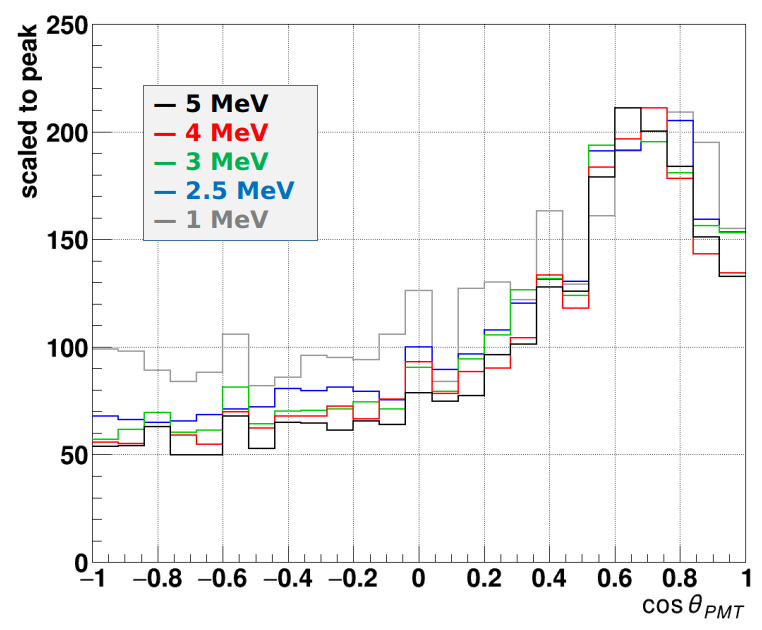
\includegraphics[width=8cm]{cherenkov_scint_variousE.png}
	\caption{Distributions of $\cos\theta_{PMT}$ after the prompt time cut for various $e^-$ energies simulations.}
	\label{cherenkov_variousE}
\end{figure}







\begin{figure}[!htb]
	\centering
	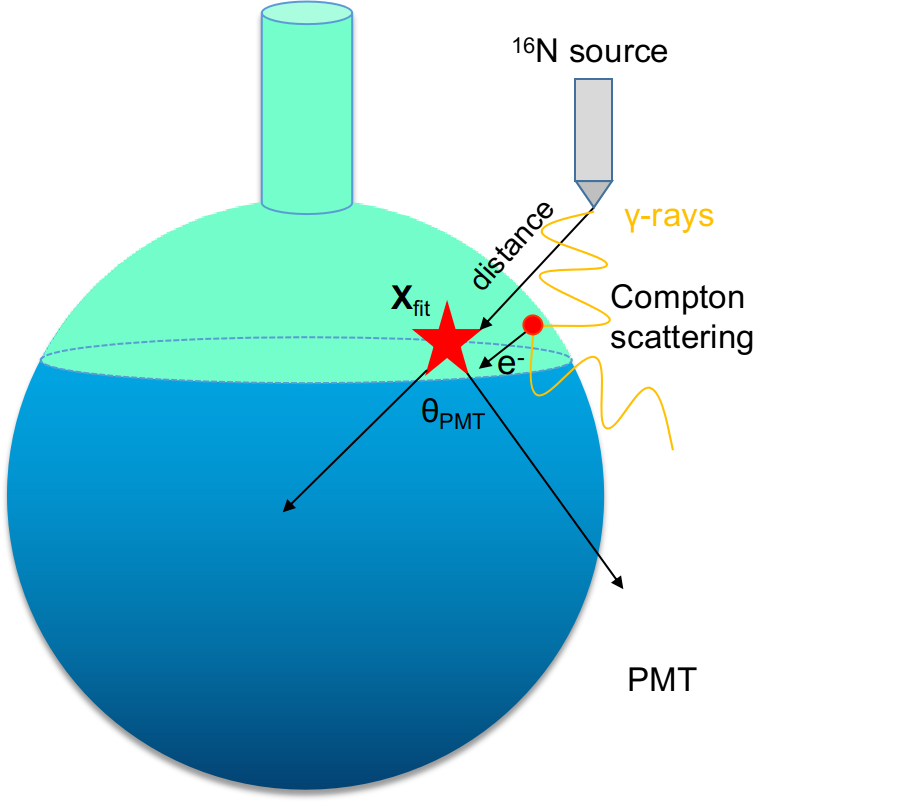
\includegraphics[width=6cm]{partialN16.png}
	\caption{$\isotope[16]{N}$ source calibration in external water during the partial-fill phase.}
	\label{partialN16}
\end{figure}


\subsubsection{$\isotope[16]{N}$ Source Analysis}

$\phi=\hat{\vec{v}}_e\cdot\hat{\vec{v}}_{assume}$

$\vec{n}=\hat{\vec{v}}_e\times\hat{\vec{v}}_{assume}$
\[
R=\begin{bmatrix}
n^2_x(1-\cos\phi)+\cos\phi       &n_xn_y(1-\cos\phi)-n_z\sin\phi & n_xn_z(1-\cos\phi)+n_y\sin\phi \\
n_xn_y(1-\cos\phi)+n_z\sin\phi & n^2_y(1-\cos\phi)+\cos\phi & n_yn_z(1-\cos\phi)-n_x\sin\phi \\
n_xn_z(1-\cos\phi)-n_y\sin\phi & n_yn_z(1-\cos\phi)+n_x\sin\phi & n^2_z(1-\cos\phi)+\cos\phi
\end{bmatrix}
\]
$\vec{v'}_e=R\vec{v}_e$

$\vec{X'}_{evt}=R\vec{X}_{evt}$

Move $\vec{X'}_{evt}$ to the origin,

$\vec{X'}_{pmt}=R\vec{X}_{pmt}-\vec{X'}_{evt}$

Breit-Wigner function
\[
p(x) = \frac{c_0}{\pi}\frac{\frac{1}{2} \Gamma}{(x-m)^2 + (\frac{1}{2} \Gamma)^2}+c_1
\]

\subsubsection{$AmBe$ Source Analysis}









\section{Relative Light Yield Measurements of the Te-loaded Liquid Scintillators}

If the predicted process of 0νββ-decay exists,  the tellurium isotope will undergo the process: 130Te→130Xe+2e-, where two electrons are emitted from the nuclei.  These two energetic electrons will pass through the liquid scintillator (such as LAB) and deposit energy to excite the molecules of the scintillator. When the molecules de-excite, fluorescence light is released. This process is called scintillation [cite birks, leo, knoll, markchen]. The fluorescence light can be detected by the photosensors designed for particle physics experiments. The photosensors, typically used are photomultiplier tubes (PMTs) [cite pmt], can convert the light into photoelectrons (p.e.) and the p.e.s are further magnified into measurable electrical signals. By measuring the amount of the fluorescence light, the energy of the particle from a certain process can be inferred. To measure the summed energy spectrum of the two electrons is the major task for a particle physics experiment searching for the possible 0νββ-decay signal.

For the \isotope[130]{Te} 0νββ-decay process, the signature energy peak is at $2.5~MeV$ [cite whitepaper].  This peak is relatively small and can be immerged in the ubiquitous radioactive decays from natural sources, such as the natural Uranium and thorium decay chains existing in the materials [cite whitepaper]. Therefore, the 0νββ-decay experiments require a very high energy resolution to distinguish the signal from the backgrounds. For the liquid scintillator, it is expected to create as large amount of light caused by a particle interaction as possible. A quantity of light yield, defined as the number of photons for per MeV energy deposit (photons/MeV) by a particle interaction, is used for describing the detection property of the liquid scintillator.

An additional wavelength shifter, 2,5-diphenyloxazole (PPO) is usually added and dissolved into the LAB [cite ppo]. This wavelength shifter is used as a fluor and it can shift the wavelengths of the scintillation photons to a range of 300-550 nm, which is the sensitive range of the PMT detection.  A 2 g/L PPO concentration in LAB is optimized by SNO+ [cite whitepaper]. The absolute light yield of the LAB-PPO liquid scintillator has been well-measured from large particle physics experiments [cite dayabay, borexino] as well as bench-top measurements [cite dayabayBench, novikov, tanner]. The absolute light yield of LAB+2g/L PPO liquid scintillator determined by SNO+ is 11900 photons/MeV [cite lightyield].

In this paper, we measured the light yield of $0.5\%$ Tellurium loaded LAB (TeLS) samples relative to the LAB-PPO scintillator (relative light yield, RLT). With tellurium loading into the LAB, the light yield of the liquid scintillator will go down since the tellurium atoms can block the photon transmissions to the photosensors.  The light yield of the TeLS is crucial for the 0νββ-decay experiments since it determines the energy resolution. It is also crucial for the experiments that are aimed to develop high light yield Tellurium-loaded scintillators [cite stevebiller].

\subsection{Measurement Setup and Data Acquisition}

We first prepared LAB+2 g/L PPO by dissolving PPO into the pure LAB. The LAB-PPO mixture was distilled by heating and flowing with liquid nitrogen to remove humidity and oxygen, which can affect the light yield, for 48 hours. The distilled LAB-PPO was added into the original 16.5\% weight Te-butanediol samples to dilute into the 0.5\% TeLS samples.  Te-butanediol samples from both of the DDA and SOP synthesis procedures are prepared and are referred as TeDDA and TeSOP samples respectively. These samples are further transferred into scintillation vials for the measurement. These vials have PTFE caps sealed on the top of the glass cylinders. To avoid air bubbles created by squeezing the vial cap into the liquid, the liquid level for each sample is kept at 30 mm. The dimensions of the vial is shown in the left picture of Fig.~ 12.

Two Hamamatsu R580 PMTs [cite PMT] were used for detecting the light. The diameter of the PMT round surface is 38.71 mm. These PMTs were housed in stainless steel cylinders (PMT holders), set face to face, looking at the scintillation vial from each side. The PMTs and the vial were aligned by a plastic piece, as shown in the right picture in Fig.~12.  The plastic piece is in a cylindrical shape with a hole on the top to plug in the scintillation vial and a slot at the bottom to attach a radioactive source. Inside the cylinder, there is a button-shaped groove at the bottom to fix the vial plugged in and keep the vial upright. Also, a 2-mm-diameter hole was drilled at the bottom of the piece to allow the radiation rays to go inside from the bottom. The surface inside was polished to reduce the absorption of the material to the photons. The piece is made of plant-based and biodegradable PLA filament and was machined by 3D-printing facility. The pictures of the piece are shown in Fig.~ 13.

Fig.~ 14 shows a diagram of the whole measurement setup. The plastic piece held the radioactive source and the scintillation vial. It also aligned two PMTs to face to the scintillation vial from each side. The piece can shield lights from outside as well. These setups were placed in a dark box to prevent the lights from lab. Two RG59/U type high voltage (HV) cables connected the PMTs to an HV supply outside the dark box. The HV cables were connected to two signal/HV split boxes to separate the HV current and electrical signals. Due to the resistor of the split box, the HV supply was set to 2200 Volts (V) for the PMT operation while the operation voltage suggested by the Hamamatsu is 1800 V. 

The signal cables from the split box were connected to a two-channel Hewlett Packard (HP) amplifier. The amplified signals were then input into a two-channel digitizer. The digitizer records the data and sent them to a desktop computer.

To obtain and analyze the data, we used a desktop Waveform Digitizer, the DT5751 module provided by the Costruzioni Apparecchiature Elettroniche Nucleari S.p.A (CAEN). Running at a digital pulse processing mode, the module records the digitized PMT waveforms with a data-taking rate of 1 GHz for each channel [cite CAEN].

This module is controlled by the CoMPASS software, which is provided by CAEN. The software sets up the threshold and trigger parameters. For each triggered event which passes the threshold, the software records event time, trigger flag and waveform histograms from the two channels. By integrating the waveforms, it can also calculate the energy of a triggered event [cite compass].

Each channel recorded the signals from each PMT individually. With the two-PMT setup, we applied coincidence time mode measurements. In the coincidence mode, a coincidence time window between two channels were set to 48 ns. For a certain event, the CoMPASS software compares the event time difference between two channels and only records it if the event time differences is less than 48 ns. A smaller window of 10 ns was further applied for analysis.


Fig.~12: Test sample (left) and setup (right). Left: The samples were filled into scintillation vials. The dimensions are shown in the picture. Right: Two PMTs are aligned to face to the scintillation vial from each side.


Fig.~ 13. The plastic piece holds the radiation source and the scintillation vial.  It also aligns the PMTs to face the vial from two sides.
Fig.~ 14:  Diagram for the light yield measurement setup. See the text for details.

Measurement

The liquid scintillator samples we have measured are: LAB-PPO, TeDDA, TeSOP. The unloaded LAB-PPO sample served as a standard candle. 


A Cesium-137 (\isotope[137]{Cs}) radioactive source was always placed at the bottom of the scintillation vials.
The source was made by Radiochemical Centre Amersham. The radioactivity measured on 1st April 1974 was $11.09~microcurie(\mu Ci)$, with an accuracy of $3.7\%$. The activity was expected to be 
in this thesis, considering a half-life of 30.08 years for the \isotope[137]{Cs}\cite{nndc}.




  has a 85.10\% chance to emit 0.661 MeV $\gamma$-rays [cite nndc]. These $\gamma$-rays can travel into the liquid scintillator samples in the vial, interact with the samples and create scintillation photon.

For each sample, measurements were taken for one-minute time duration. Waveforms from the PMT photo-current signals were digitized in a 252 ns time window. Shown in Figure 15 is a typical waveform caused by γ rays interacted with the LAB-PPO sample. For the p.e. signals, pulses formed in the waveform. For each waveform, the digitizer firmware dynamically calculated the baseline as the mean value of 256 data points inside a moving time window of 252 ns. A threshold was set as 100 units above the baseline. The data point on the 90\% leading edge of the pulse was taken as the trigger time tag. From this trigger time tag, in the following 80 ns window the digitizer did not calculate another trigger to avoid introducing another pulse (trigger hold-off). Also from the trigger time tag, a pre-gate of 8 ns was set. The waveform was integrated in the time gate of  [trigger time - 8,  trigger time + 72] ns. This gives the integrated charge, which was calculated as a A/D converter (ADC) channel number. If the measurement system can be calibrated, the ADC channel number can be exactly converted into the energy of the particle interaction. Since here we only interested in the photon numbers, we simply used ADC channel as the energy. Once the pulse in the waveform passed the threshold and a triggered time tag can be found, the digitizer considered it as a triggered event. A time flow started when the measurement began. Time stamps were recorded as event time when the triggered event hapfpened. The waveform was recorded and the ADC channel number (energy) of this event was calculated.


Figure 15.  A typical waveform triggered by scintillation photons from 137Cs $\gamma$-rays interaction with LAB-PPO sample.

In a coincidence time measurement, the event times of the events recorded by each of the two PMTs were compared. If the event time differences between two events from each PMTs were too long, these two events were considered as random noises rather than the physics events and were not recorded. We optimized a coincidence time cut as 40 ns and set that cut during the digitizer data-taking. 


Figure 16. Measured LAB-PPO energy spectrum with and without coincidence cut on the ADC channel 0.  A threshold for counting is set by comparing the two spectrum. 

Fig.~ 16 shows the measured LAB-PPO energy spectrum with and without coincidence time cut ($10~ns$) on the ADC channel 0.  Without the coincidence time cut, there exists a zero peak, which is caused by the pulses from random electronic noises or fluctuations of the digitized waveforms. The peak on the left is the single p.e. peak. It is mainly caused by some light sources which are weak enough that the photons only strike out at most one single p.e. inside the PMT [cite leo].  The peak on the right is the multiple p.e. peak, in our case is mainly caused by a number of scintillation photons produced by the γ-ray interacting with the LAB-PPO. In the coincidence time measurement mode, it only records the photons detected by the two PMTs almost simultaneously. Therefore, the zero peak is removed while the single p.e. peak is suppressed. The multiple p.e. peak is consistent with the non-coincidence measurement.  A threshold in energy can be set to count only the scintillation photons emitted from LAB-PPO. 


Fig.~ 17. A 2D energy spectrum of LAB-PPO sample, after a 10-ns coincidence window cut between two channels. The colour scale is for the counted number of events. The single p.e. and multiple p.e. peaks are also shown.

Fig.~ 17 shows the result of one-minute measurement for the LAB-PPO sample. The data points in the 2D plot represent the triggered event fall in certain ADC channel numbers in each channel. A 10 ns coincidence window cut was applied to cut down noise, single p.e. and background events. The events of the 0 ADC channel numbers, which represent noises, were totally cut off after applying the coincidence. Fig.~ 18 shows the results of the TeSOP and TeDDA samples.  Compared to the LAB-PPO sample, a shift of the multiple p.e. peak due to the different light yields between the samples can be observed clearly.



Fig.~ 18. 2D energy spectrum of the counting measurements of TeSOP (left) and TeDDA (right) samples, after a 10-ns coincidence window cut between two channels.



Fig.~ 18. Project the 2D plots onto channel 0.

In Fig.~ 18, the 2D plots in Fig.~ 17 are projected onto a single channel. We used an empty vial and let γ-rays from 137Cs source pass through it for a background run (without the coincidence cut). This is to verify the single p.e. peak and noise region, shown as the black background spectrum.

From this plot, the single p.e. peaks for all the samples as well as the background match together. The multiple p.e. peaks indicate the different light yields of the scintillator samples. Here we can clearly see the multiple p.e. peak of the LAB-PPO occupies the largest ADC channel number, while the channels of TeSOP is slightly larger than the TeDDA. 

To quantify the light yield differences between different samples, an analysis method of charge weighted photon number has been applied as the following:

First, from the spectrum, fit the single p.e. peak with an asymmetric Gaussian function, as shown in Fig.~ 19. The mean value of the asymmetric Gaussian represents the ADC channel number corresponding to the single p.e. peak.

$\xi=-\frac{\alpha(x-\mu)}{\sqrt 2\sigma}$,
$f_{asym}=c\cdot e^{-\frac{1}{2}(\frac{x-\mu}{\sigma})^2}\cdot Erfc(\xi)$

$p_0=\mu,p_1=\sigma,p_2=\alpha, p_3=c$ 


Then for the multiple p.e. region, weighting (dividing) the counts of the event in each channel with the single p.e. ADC channel number to calculate the total number of the photons.


Fig.~ 19. Fit the single p.e. peak with an asymmetric Gaussian function (fasym) to obtain the adc channel for weighting. The mean value of p0 is used as the adc channel relative to a single p.e. peak.

To define the multiple p.e. region for the counting, the spectrum projected on each channel with and without coincidence cut are compared to define a threshold of the ADC channel for counting. By integrating from this threshold, the total numbers of events between two spectrum are close to each other. From two channels, we get two thresholds and then define a box cut in the 2D coincidence plot. We weights the events in the box to obtain the total number of photons. Fig.~ 16 and Fig.~ 19 show the case of the LAB-PPO sample.


Fig.~\ref{2dplot} 2D LABPPO spectrum with coincidence cut. A box cut is defined for multiple PE counting. 

Once the total number of the photons for a certain sample is counted, we can calculate its ratio to the LAB-PPO sample to obtain the relative light yield.

Results

Table 1. Number of photons calculated by Charge weighted photon number method.
sample	Number of photons (x106)	Ratio to the LABPPO
LABPPO	2.0811	1 
TeDDA	1.2652	0.61
TeSOP	1.3976	0.67

Table 1 shows the number of photons calculated by Charge weighted photon number method.

Here we quantify the relative light yields of our samples. The light yield of the $0.5\%$ Te by SOP synthesis procedure (TeSOP) is $0.61$ and the one of the $0.5\%$ Te by DDA procedure is 0.67. The light yield of TeSOP is slightly larger than the TeDDA. In [cite billerTe],  a relative light yield of ~0.65 was reported.


%[markchen] Shimizu, Itaru, and Mark Chen. "Double beta decay experiments with loaded liquid scintillator." Frontiers in Physics 7 (2019): 33.
%
%[birks] Birks, John Betteley. The theory and practice of scintillation counting: International series of monographs in electronics and instrumentation. Vol. 27. Elsevier, 2013.
%
%[leo] Leo, William R. Techniques for nuclear and particle physics experiments: a how-to approach. Springer Science & Business Media, 2012.
%
%[knoll]Knoll, Glenn F. Radiation detection and measurement. John Wiley & Sons, 2010.
%
%[novikov] V. Novikov, Scintillator development for SNO+, SNO+ internal document (2009).
%
%[pmt] “Photomultiplier Tube R580.” Photomultiplier Tube R580 | Hamamatsu Photonics, www.hamamatsu.com/eu/en/product/type/R580/index.html. 
%
%
%[ppo] Wunderly, Stephen W., and Joel M. Kauffman. "New quench-resistant fluors for liquid scintillation counting." International Journal of Radiation Applications and Instrumentation. Part A. Applied Radiation and Isotopes 41.9 (1990): 809-815.
%
%[whitepapter] Andringa, S., et al. "Current status and future prospects of the sno." Advances in High Energy Physics 2016 (2016).
%
%[dayabay] W. Beriguete. et al., Production of Gadolinium-loaded Liquid Scintillator for the Daya Bay Reactor Neutrino Experiment, arXiv:1402.6694 [physics.ins-det]
%
%[dayabayBench] Xing-Chen, Ye, et al. "Preliminary study of light yield dependence on LAB liquid scintillator composition." Chinese Physics C 39.9 (2015): 096003.
%
%[tanner] Kaptanoglu, Tanner, Meng Luo, and Josh Klein. "Cherenkov and scintillation light separation using wavelength in LAB based liquid scintillator." Journal of Instrumentation 14.05 (2019): T05001.
%
%[lightYield] S. Grullon. Light yield and scintillation decay time constants of Te-loaded liquid scintillator for the SNO+experiment. InProceedings ofthe 26th International Conference on Neutrino Physics and Astrophysics(Neutrino ’14), Boston, MA, June 2014. Boston University.
%
%[stevebiller] Biller, Steven, Szymon Manecki, and SNO+ collaboration. "A new technique to load 130Te in liquid scintillator for neutrinoless double beta decay experiments." Journal of Physics: Conference Series. Vol. 888. No. 1. IOP Publishing, 2017.
%
%[caen] “DT5751 - CAEN - Tools for Discovery.” CAEN, www.caen.it/products/dt5751/.
%
%[compass]  “CoMPASS Multiparametric DAQ Software for Physics Applications
%”https://www.caen.it/products/compass/
%
%[nndc] Decay Radiation Results, Brookhaven National Laboratory, www.nndc.bnl.gov/nudat2/decaysearchdirect.jsp?nuc=137CS&unc=nds.
%
%[billerTe] Biller, Steven, Szymon Manecki, and SNO+ collaboration. "A new technique to load 130Te in liquid scintillator for neutrinoless double beta decay experiments." Journal of Physics: Conference Series. Vol. 888. No. 1. IOP Publishing, 2017.

